\section{Introduction}
\label{sec:intro:0}

The Vera C. Rubin Observatory’s Data Preview 1 (DP1) marked an important milestone in preparing for the forthcoming Legacy Survey of Space and Time (LSST), offering a valuable opportunity to test and validate scientific tools and workflows on precursor imaging data. Among the core scientific objectives of LSST is the estimation of photometric redshifts (photo-zs) for billions of galaxies, enabling cosmological analyses that rely on redshift-dependent distributions. In the context of DP1, the "Photoz Science Unit" was tasked with generating robust photometric redshift estimates using the available multi-band imaging, laying the groundwork for future large-scale applications. This effort required integrating realistic data processing with scalable machine learning techniques capable of delivering precise redshift predictions across varied galaxy populations.

To carry out this task, the Photoz Science Unit employed the RAIL (Redshift Assessment Infrastructure Layers) software package, a flexible and modular platform specifically designed for photometric redshift estimation and evaluation. RAIL supports a range of machine learning and template-fitting algorithms and offers streamlined pipelines for training, testing, and applying photo-z models. For DP1, the team used RAIL to train supervised machine learning models on spectroscopic datasets that had been carefully matched to the DP1 photometric catalog. These training sets included galaxies with known spectroscopic redshifts, providing ground truth labels essential for optimizing model performance and assessing predictive accuracy.

A critical step in the process involved constructing a reliable and representative training sample. The matched spectroscopic datasets were drawn from several publicly available surveys that overlapped with the DP1 sky coverage, including deep fields with multi-band photometry similar to that expected from LSST. These spectroscopic redshifts enabled the calibration of photometric inputs, such as magnitudes, colors, and potentiall morphological features, against measure spectroscopic redshift values, allowing the machine learning models within RAIL to learn meaningful mappings between observed photometric properties and cosmological distance.  The performance of the trained models was evaluated using metrics such as bias, scatter, and outlier fraction, ensuring that the outputs met quality standards suitable for scientific analysis.

The outcome of this effort was a set of photometric redshift estimates that are demonstrative of the pipeline's readiness for larger-scale deployment in future data releases.  The collaboration between the Photoz Science Unit and the broader DP1 effort provided valuable feedback on data quality, training requirements, and model generalization, while highlighting the importance of high-quality spectroscopic training sets. Moreover, the use of RAIL established a reproducible and extensible framework for photo-z estimation that can evolve in parallel with LSST’s data volume and complexity. This initial deployment in DP1 thus serves as a prototype for future photometric redshift workflows in the LSST era.

\section{Data}
\label{sec:data:0}

\subsection{Rubin DP1}
\label{sec:data:dp1}

The Rubin Observatory’s Data Preview 1 (DP1) dataset is the first public release of real imaging data processed through the LSST Science Pipelines, serving as a critical testbed for scientific and technical validation ahead of full LSST operations.  DP1 is based on observations from the LSST commisioning camera (LSSTComCam) and includes multi-band optical imaging (typically in u, g, r, i, z and y filters) over several square degrees of sky.  The dataset consists of processed images, source catalogs, and associated metadata, all formatted using the Rubin Data Butler system to simulate LSST-like data products. Although smaller in scale than future LSST datasets, DP1 offers realistic photometric measurements, object detection, and data structures, making it an invaluable resource for developing and testing algorithms for tasks such as photometric redshift estimation, object classification, and data quality assessment.

\subsection{Reference Sample}
\label{sec:data:reference}



\subsubsection{Euclid Spec-z dataset}
\label{sec:data:euclid}

\begin{figure*}
    \centering
%    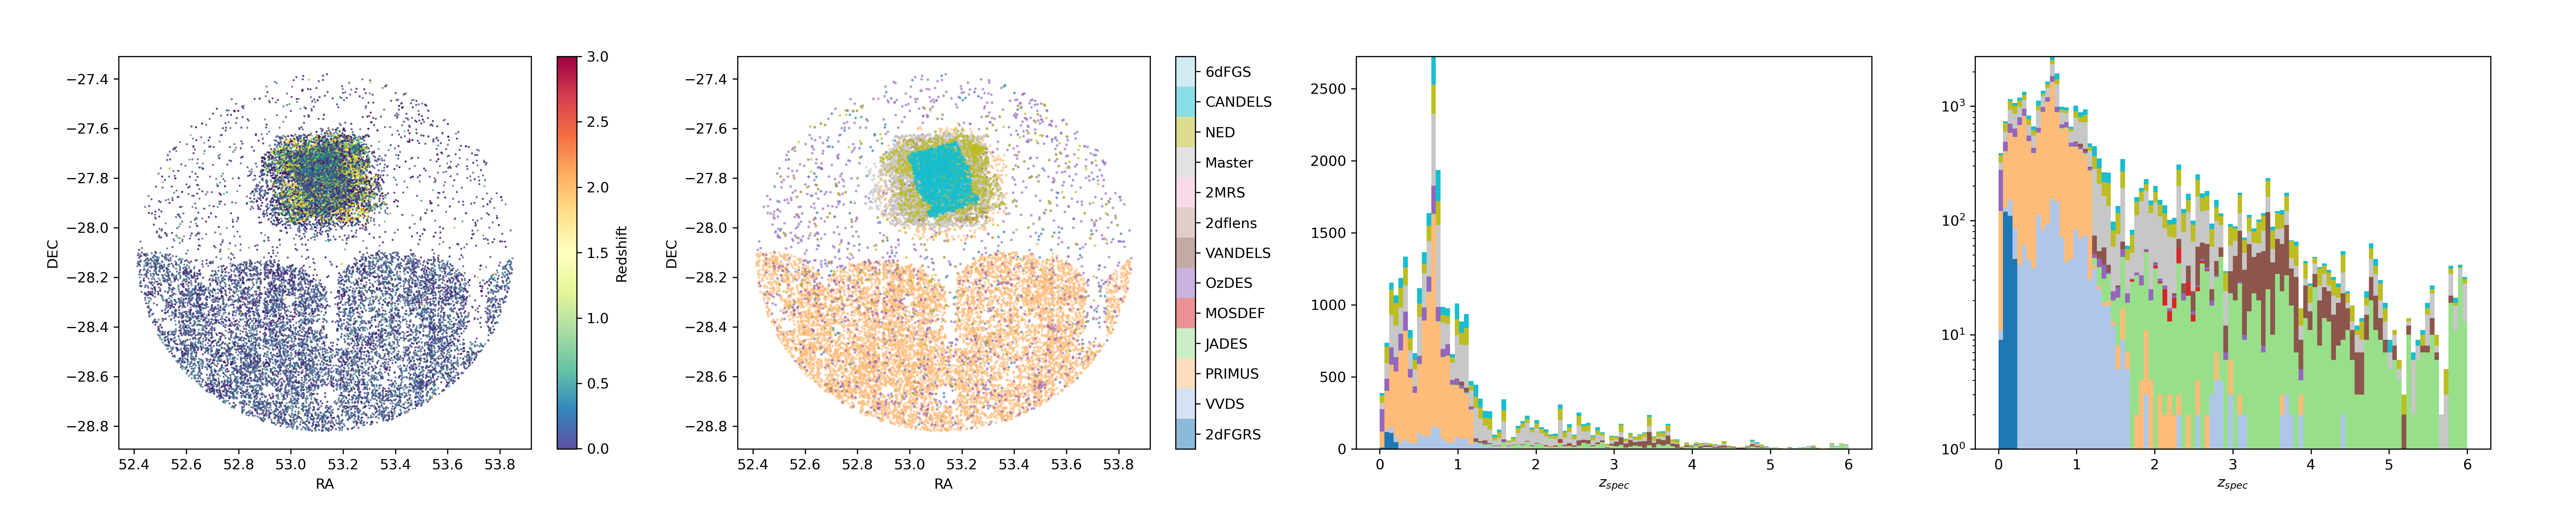
\includegraphics[width=1.0\linewidth]{figures/training_set_info.png}
    \caption{Training set in the ECDFS field. Panel 1: Scatter plot of the ECDFS reference catalog color coded by redshift. Panel 2: scatter plot of the ECDFS reference catalog color coded by the survey name. Panel 3 and Panel 4: redshift distribution with y-axis in linear and log scale. }
    \label{fig:enter-label}
\end{figure*}

\subsubsection{DESI DR1}
\label{sec:data:desi}


\section{Methodology}
\label{sec:method:0}

To produce photometric redshift estimates for the Rubin DP1 dataset, the Photoz Science Unit used the RAIL (Redshift Assessment Infrastructure Layers) software package as the core tool for training, evaluating, and applying photometric redshift estimation models. RAIL provides a modular and extensible framework that integrates a variety of machine learning and template-fitting algorithms, along with standardized interfaces for data input, model training, prediction, and validation. For the DP1 effort, RAIL was configured to use the multi-band photometric measurements from the DP1 object catalogs as input features—typically including magnitudes and colors derived from the g, r, i, and z bands.

The photo-z models were trained using spectroscopic datasets that were matched to DP1 photometric sources, serving as labeled examples with known redshifts. RAIL's pipeline handled the ingestion of these training datasets, preprocessing steps such as feature normalization and selection, and the training of supervised learning models such as random forests, k-nearest neighbors, or neural networks. Once trained, these models were applied to the full DP1 photometric catalog to generate redshift predictions for galaxies without spectroscopic coverage.

RAIL also supported evaluation of the model performance through a suite of diagnostic metrics, including redshift bias, scatter (e.g., normalized median absolute deviation), and catastrophic outlier rate. These evaluations were performed using held-out validation sets or cross-validation strategies to ensure robustness and generalizability. The entire workflow—from data ingestion and training to inference and validation—was conducted within RAIL’s reproducible and scalable infrastructure, allowing the Photoz Science Unit to produce scientifically meaningful photometric redshift estimates and to assess their quality within the context of Rubin’s early data products.

\subsection{Template fitting based}
\label{sec:method:template}


\subsection{Machine Learning based}
\label{sec:method:machine_learning}

\subsection{Bookkeeping software}
\label{sec:method:rail_project}
